\documentclass[conference]{IEEEtran}

%
% Block Breaker Game based on NIOS-II Soft Processor
% \^O^/
% \^V^/
% \^W^/
% 

\usepackage{pxrubrica}
\usepackage[pdftex]{graphicx}
\usepackage{amsmath}
\usepackage{algorithmic}
\usepackage{array}
\usepackage{fixltx2e}
\usepackage{stfloats}
\usepackage{anyfontsize}
\usepackage{url}
\usepackage{multirow}
\usepackage{multicol}
\usepackage{textcomp}
\usepackage{float}
\usepackage{wrapfig}
\usepackage{listings}
\usepackage{pifont}
\usepackage{tikz}
\usepackage{parskip}
\usepackage{amssymb}

% ?
\ifCLASSOPTIONcompsoc
  \usepackage[caption=false,font=normalsize,labelfont=sf,textfont=sf]{subfig}
\else
  \usepackage[caption=false,font=footnotesize]{subfig}
\fi

\title{
    Block Breaker Game based\\on NIOS-II Soft Processor \\ 
    \emph{ENGI-9865: Report of Course Design}
}

\author{
    \IEEEauthorblockN{
        Jiabao Guo
    }
    \IEEEauthorblockA{
        Student Number: 202096888 \\
        jiabaog@mun.ca \\
        Memorial University of Newfoundland
    }
}

\begin{document}
\maketitle

% Display page number.
\thispagestyle{plain}
\pagestyle{plain}

\begin{abstract}
Targeting to the DE-10 Stadnard FPGA board, an attempt has been made to implement a Block Breaker video game based on the NIOS-II Soft Processor, using VGA port to output video data. This report also discussed in detail including the design of the architecture, the hardware and software implementation, state transition, and the performance and two profilling methods of the final work. In addition to the profiling methods, the authors also introduced the use of TCL scripts to realize the automatic QuestaSim test report generation, and a new simple testing using pure C and standard IO that is compatible with an embeded development environment.
\end{abstract}

\textbf{\textit{Keywords}---}DE-10; FPGA; NIOS-II; Video Game; Block Breaker; VHDL; ASIC; Embedded Development

% For peer review papers, you can put extra information on the cover
% page as needed:
% \ifCLASSOPTIONpeerreview
% \begin{center} \bfseries EDICS Category: 3-BBND \end{center}
% \fi
%
% For peerreview papers, this IEEEtran command inserts a page break and
% creates the second title. It will be ignored for other modes.
%\IEEEpeerreviewmaketitle

\tableofcontents

%%%%%%%%%%%%%%%%%%%%%%%%%%%%%%%%%%%%%%%%%%%%%%
%%%%%%%%%%%%%%%%%%%%%%%%%%%%%%%%%%%%%%%%%%%%%%
%%%%%%%%%%%%%%%%%%%%%%%%%%%%%%%%%%%%%%%%%%%%%%
%%%%%%%%%%%%%%%%%%%%%%%%%%%%%%%%%%%%%%%%%%%%%%
%%%%%%%%%%%%%%%%%%%%%%%%%%%%%%%%%%%%%%%%%%%%%%
%%%%%%%%%%%%%%%%%%%%%%%%%%%%%%%%%%%%%%%%%%%%%%
%%%%%%%%%%%%%%%%%%%%%%%%%%%%%%%%%%%%%%%%%%%%%%
%%%%%%%%%%%%%%%%%%%%%%%%%%%%%%%%%%%%%%%%%%%%%%
%%%%%%%%%%%%%%%%%%%%%%%%%%%%%%%%%%%%%%%%%%%%%%
%%%%%%%%%%%%%%%%%%%%%%%%%%%%%%%%%%%%%%%%%%%%%%
%%%%%%%%%%%%%%%%%%%%%%%%%%%%%%%%%%%%%%%%%%%%%%
%%%%%%%%%%%%%%%%%%%%%%%%%%%%%%%%%%%%%%%%%%%%%%

\section{Introduction}

This project is mainly consist of the concept of the ``Block Breaker'' game and the application of NIOS-II Soft Processor that targeted to the DE-10 Standard Altera FPGA board. To describe our work in detail, we will discuss from 3 aspects, including:

\begin{itemize}
    \item \textbf{Introduction.} In this section, we will first briefly introduce the background of this type of classic collision game, then discuss the use the NIOS-II Soft Processor to implement the game, and how our version of Block Breaker game works, and finally, from our own perspective, the reason of using the NIOS-II instead of pure VHDL. 
    \item \textbf{Architecture of Design.} In this section, we will look into the hierachy of hardware components, explaining the design of each of them, then we will show the main game logic written in C that running on the NIOS-II Soft Processor. Also, in the end of this part we will present the game state transitions including an ASM chart and a state transition table.
    \item \textbf{Profiling of Design.} In this section, an attempt has been made to not only launch the QuestaSim (the successor of ModelSim) on the hardware side of the project, but also achieve automatic test report generation (a message box \textbf{showing an overall PASS/FAIL signal for each component}, followed with a list of testcases and the PASS/FAIL status for each of them, \textbf{without having to check the waveform manually}) by one click. In addition, another attempt has been made to achieve the same thing on the software side, but with one more step that we called it \textbf{``Fake Environment''}.
\end{itemize}


\subsection{Game Background}
Block Breaker is a kind of very classic collision game. Your goal in this game is to launch the ball in the paddle (or call it tray) and break all the blocks suspended above.

\subsection{The NIOS-II}
\textbf{This subsection is mainly based on the content of the official PDF document from Altera \emph{Nios II Embedded Processor Backgrounder}, which can be found at the \cite{bib_nios2} of reference.}

\subsubsection{Key Features}
The Nios II architecture is a RISC soft-core architecture with full 32-bit design:
\begin{itemize}
    \item 32 general-purpose 32-bit registers,
    \item Full 32-bit instruction set, data path, and address space,
    \item Single-instruction 32x32 multiply and divide producing a 32-bit result.
\end{itemize}

\subsubsection{CPU Family}
Nios II classic is offered in 3 different configurations: Nios II/f (fast), Nios II/s (standard), and Nios II/e (economy). Nios II gen2 is offered in 2 different configurations: Nios II/f (fast), and Nios II/e (economy).

\textbf{In this project, we are using the NIOS-II/e (economy) configuration as it does not require a license and is free for use.}

\subsection{Gameplay and Logics}
\textbf{In order to reduce the eye irritation caused by the bright sharp red color, the pictures in this section were darkened and may look blurry.}

This subsection shows the gameplay of the project. 

\begin{itemize}
    \item \textbf{In fig. \ref{fig_idle}}: Before starting the game, the digital tubes display the ``PRESS ANY KEY'' periodly, telling the player to press any button to start the game.
    \item \textbf{In fig. \ref{fig_in_game}}: The game starts and the VGA display shows the game screen as \ref{fig_gameplay}. In term of controlling the paddle, there are 4 buttons on the right bottom corner of the board. From left to right, they are: Move Left, Move Left, Move Right, Cheat, respectively. There are 2 move-lefts and 1 move-right. The extra cheat button, was another move-right, but changed temperarily for the purpose of presentation. Hitting the cheat button will force the current level to be win (pass), and the game will continue to the next level.
    \item \textbf{In fig. \ref{fig_win}}: When clearing all the blocks in the current level, The ``GOOD JOB'' text flashes for 2 times to encourage the player to continue playing. Then, the game pauses and the ``PRESS ANY KEY'' in fig. \ref{fig_idle} appears. After pressing any button, the game will continue to the next level.
    \item \textbf{In fig. \ref{fig_lose}}: If the ball fall below the paddle, then this is a fail. If you fail the level, the game displays the ``LOSE'' text and flashes for 2 times, indicating that you have lose. Then, the game pauses and the ``BETTER NEXT TIME'' in fig. \ref{fig_fail} appears, telling the player that do not be discouraged.
    \item \textbf{In fig. \ref{fig_game_clear}}: When passing all levels, the text ``GAME CLEAR'' flashes for 2 times telling the player that the game is finished. Then, the game pauses and the ``GAME OVER'' in fig. \ref{fig_game_over} appears. Then, after pressing any button, the game will restart from the first level.
\end{itemize}


\begin{figure}[h] %h
    \centering
    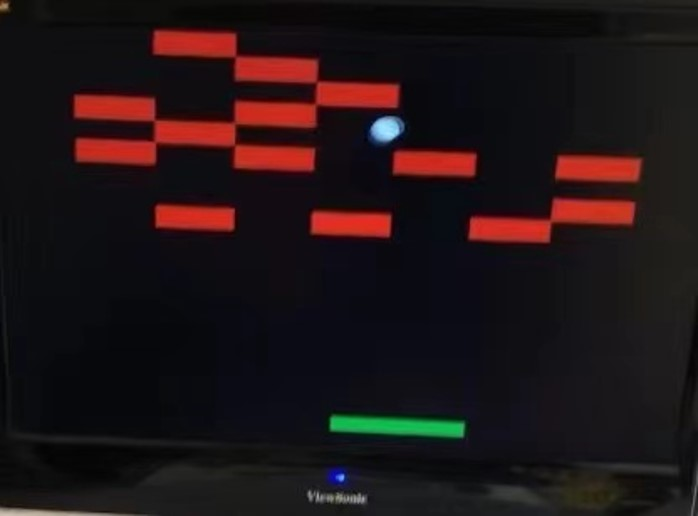
\includegraphics[width=0.45\textwidth]{imageset/diag_3}
    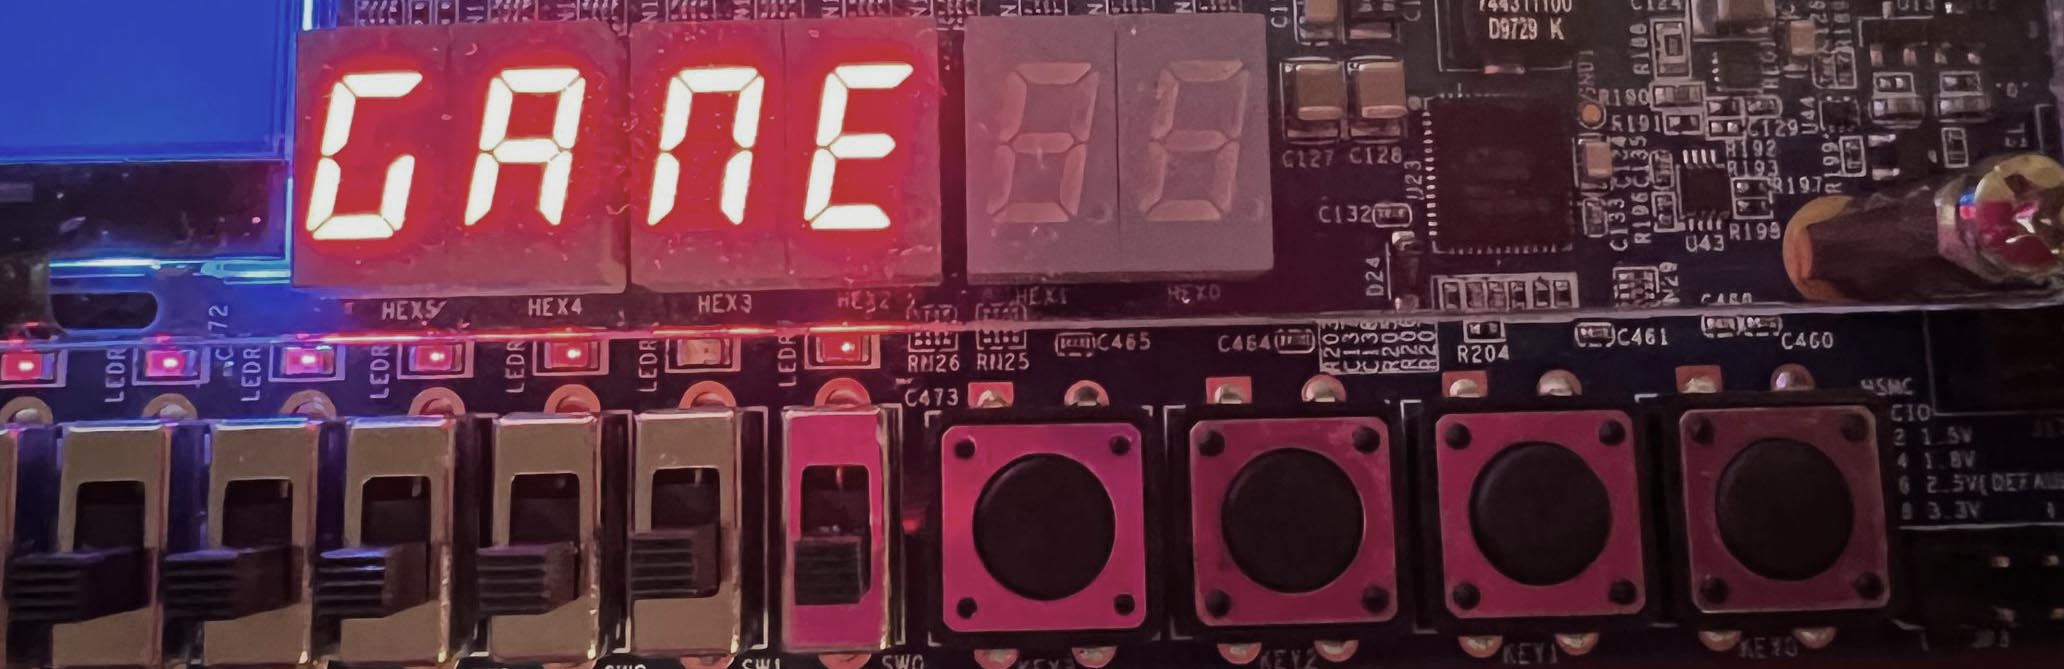
\includegraphics[width=0.45\textwidth]{imageset/buttons}    
    \caption{
        Gameplay scene at level 1\\
        There are 4 buttons on the right bottom corner of the board. From left to right, they are: Move Left, Move Left, Move Right, Cheat, respectively. \\
        There are 2 move-lefts and 1 move-right. The extra cheat button, was another move-right, but changed temperarily for the purpose of presentation. Hitting the cheat button will force the current level to be win (pass), and the game will continue to the next level.
    }
    \label{fig_gameplay}
\end{figure}

\begin{figure}[h] %h
    \centering
    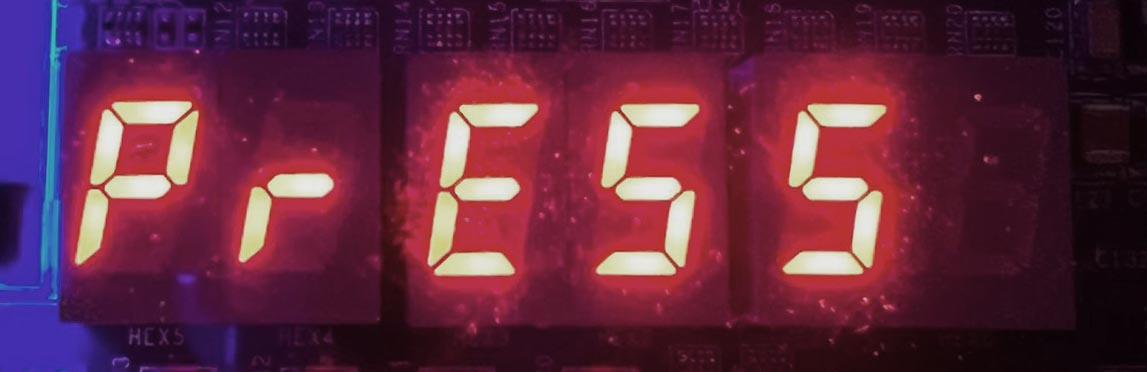
\includegraphics[width=0.45\textwidth]{imageset/press}
    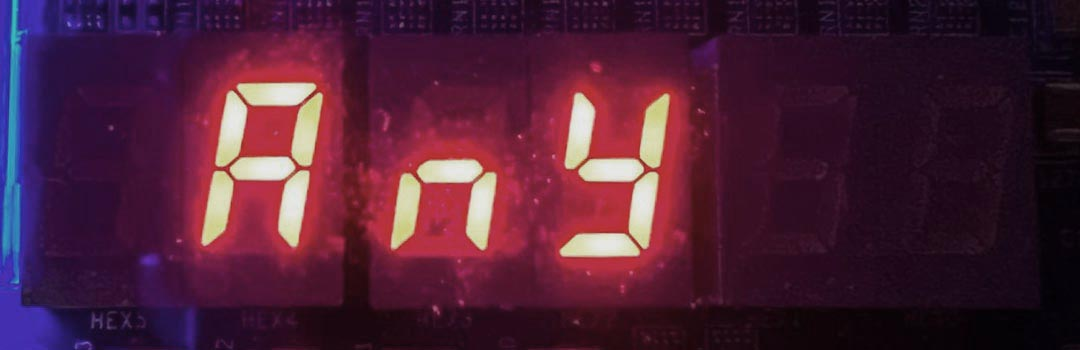
\includegraphics[width=0.45\textwidth]{imageset/any}
    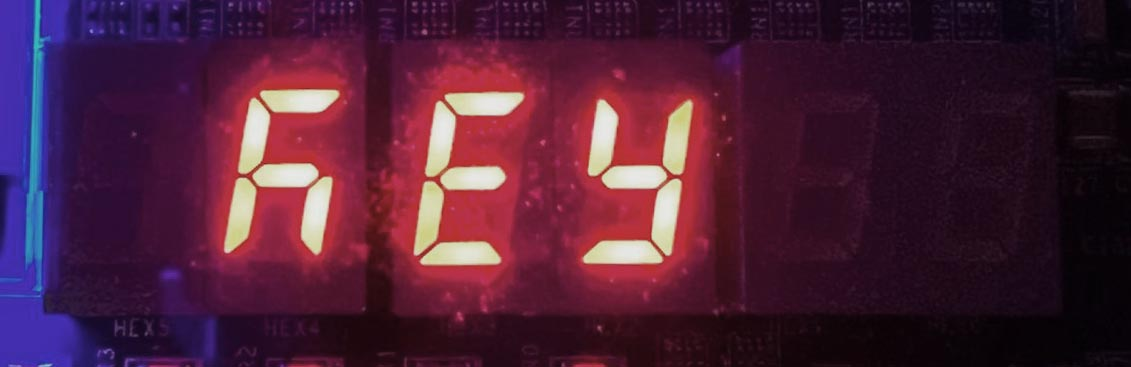
\includegraphics[width=0.45\textwidth]{imageset/key}
    \caption{Before Start Game: \textbf{``PRESS ANY KEY''}. The digital tubes display the ``PRESS'' and ``ANY'' and ``KEY'' periodly, telling the player to press any button to start/continue the game.}
    \label{fig_idle}
\end{figure}

\begin{figure}[h] %h
    \centering
    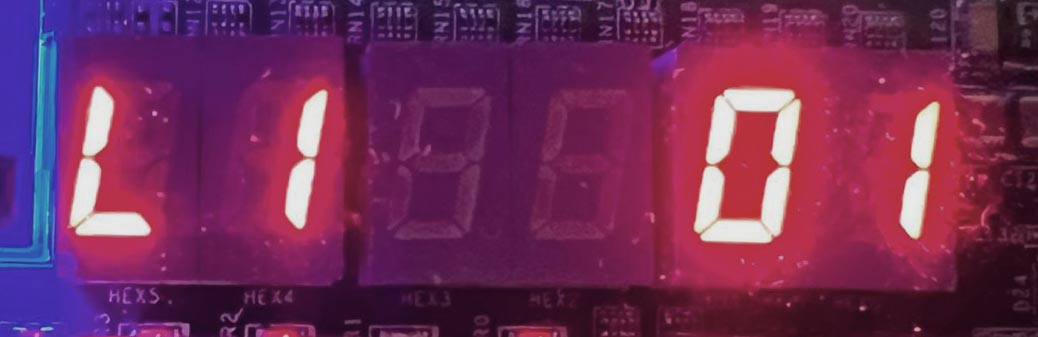
\includegraphics[width=0.45\textwidth]{imageset/level}
    \caption{In Game: \textbf{``L1 01''} means Level 1, Score 01. There are 3 levels in total. Score inherits between levels. The maximum score is 99.}
    \label{fig_in_game}
\end{figure}

\begin{figure}[h] %h
    \centering
    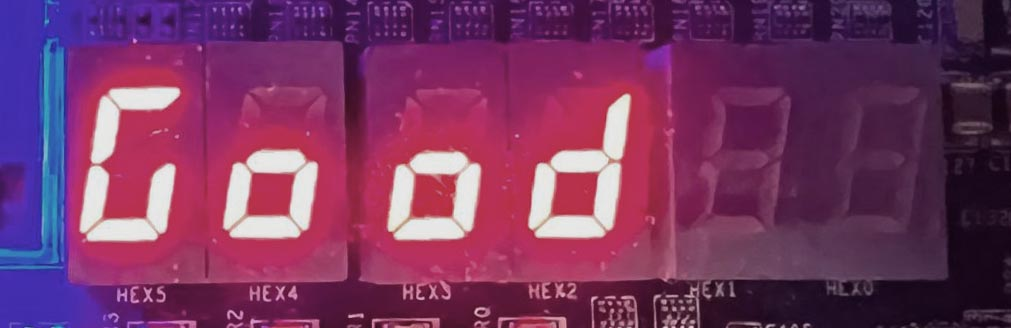
\includegraphics[width=0.45\textwidth]{imageset/good}
    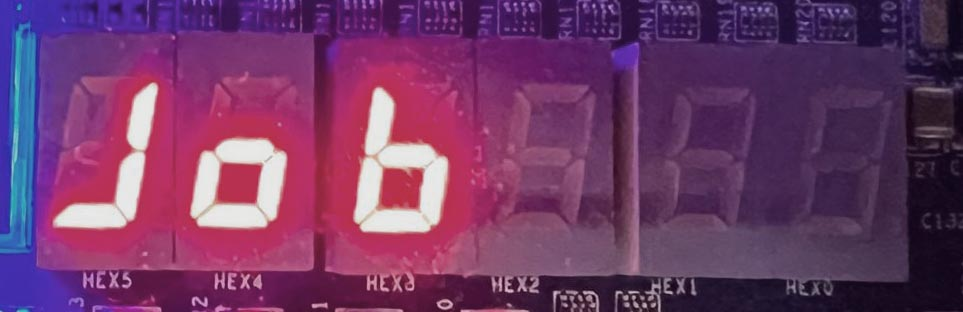
\includegraphics[width=0.45\textwidth]{imageset/job}
    \caption{Passing Level: \textbf{``GOOD JOB''}. The text flashes for 2 times to encourage the player to continue playing.}
    \label{fig_win}
\end{figure}

\begin{figure}[h] %h
    \centering
    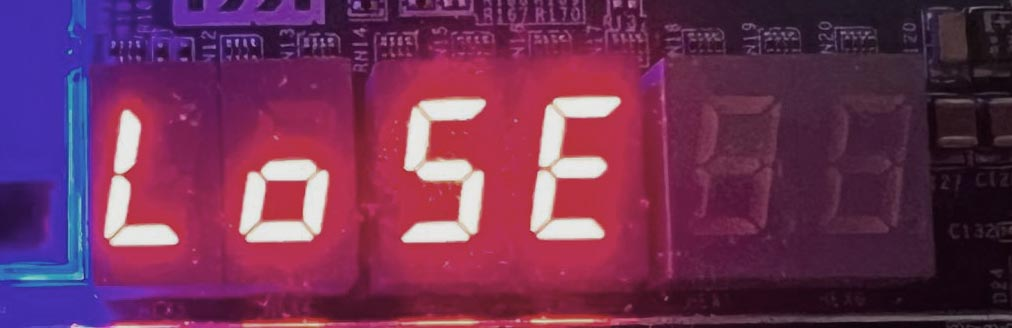
\includegraphics[width=0.45\textwidth]{imageset/lose}
    \caption{Failing Level: \textbf{``LOSE''}. The text flashes for 2 times telling the player that he or she lose the game.}
    \label{fig_lose}
\end{figure}

\begin{figure}[h] %h
    \centering
    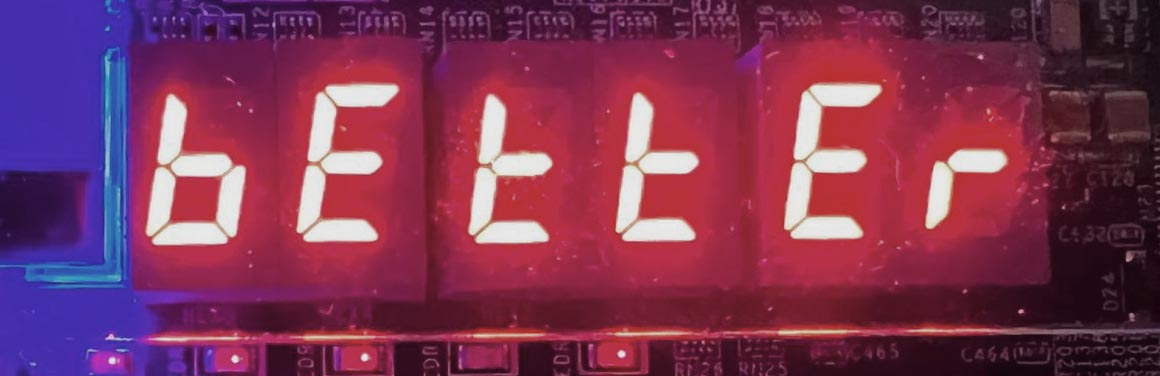
\includegraphics[width=0.45\textwidth]{imageset/better}
    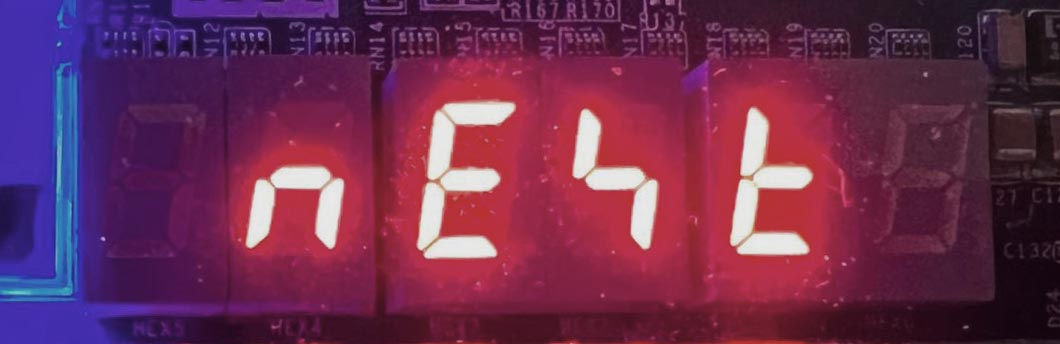
\includegraphics[width=0.45\textwidth]{imageset/next}
    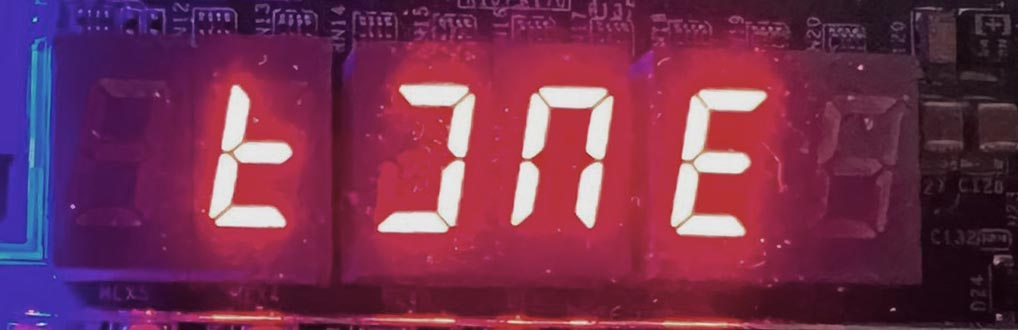
\includegraphics[width=0.45\textwidth]{imageset/time}
    \caption{Failing The Game: \textbf{``BETTER NEXT TIME''}. The text flashes for 2 times telling the player that do not be discouraged. ``BETTER NEXT TIME'' only appears after ``LOSE''.}
    \label{fig_fail}
\end{figure}

\begin{figure}[h] %h
    \centering
    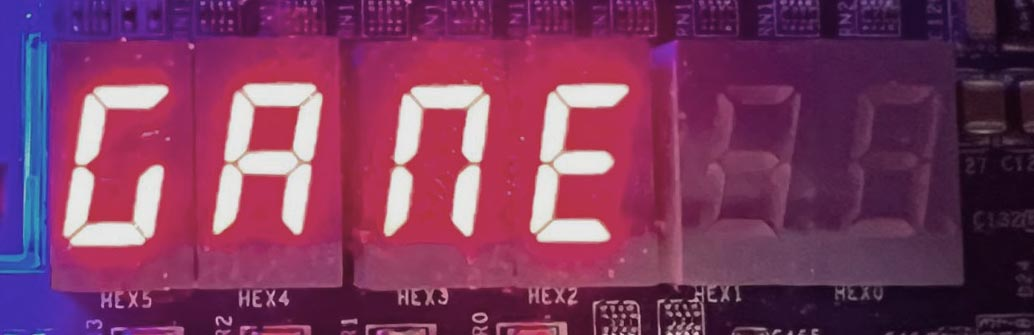
\includegraphics[width=0.45\textwidth]{imageset/game1}
    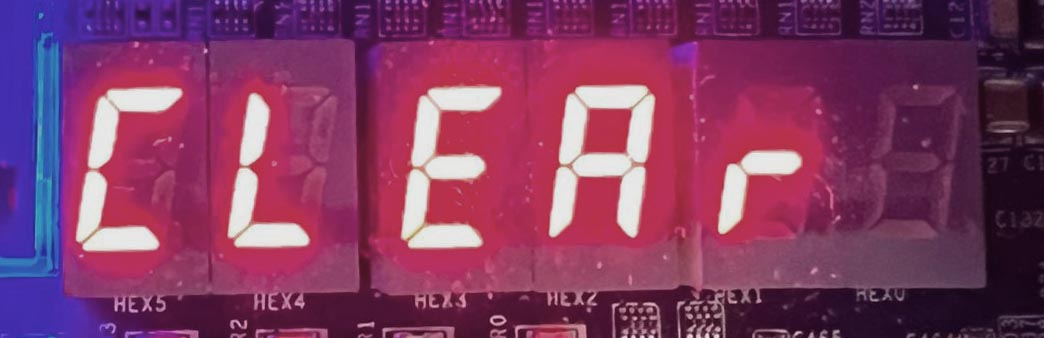
\includegraphics[width=0.45\textwidth]{imageset/clear}
    \caption{Passing all levels: \textbf{``GAME CLEAR''}. The text flashes for 2 times that express the congratulations to the player for passing all levels.}
    \label{fig_game_clear}
\end{figure}

\begin{figure}[h] %h
    \centering
    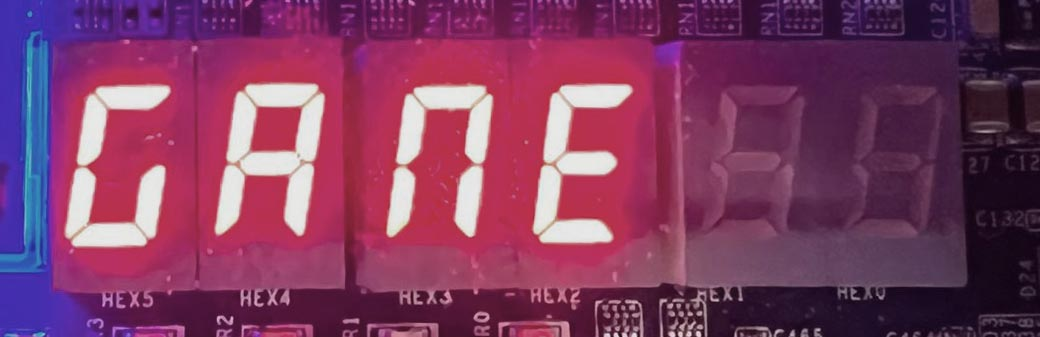
\includegraphics[width=0.45\textwidth]{imageset/game2}
    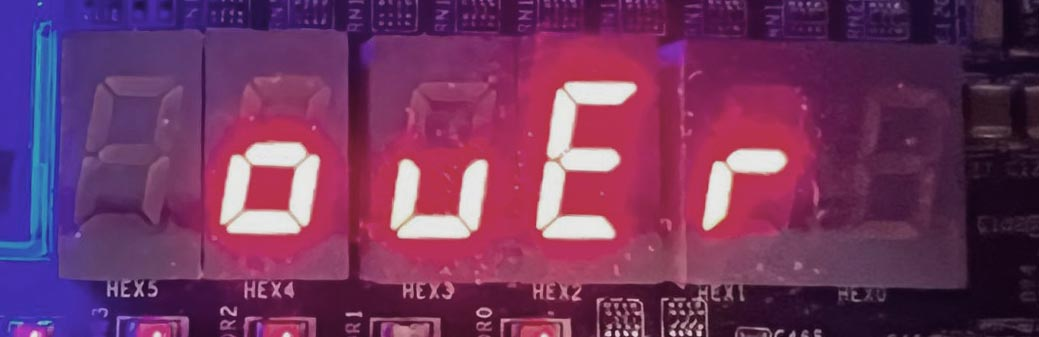
\includegraphics[width=0.45\textwidth]{imageset/over}
    \caption{Passing all levels: \textbf{``GAME OVER''}. The text flashes for 2 times indicating that the player has passed all levels and is returning to the first level now. ``GAME OVER'' only appears after ``GAME CLEAR''.}
    \label{fig_game_over}
\end{figure}

\subsection{Reasons of Using NIOS-II}
As mentioned above, the game logic is written in C instead of a HDL. As you can see, in Part C (Gameplay and Logics), the game logic is simple but with an amount of small details. For example, flashing ``Good Job'' twice for 400ms each, is extremely easy in C while requires a certain amount of time to be implemented in HDL. To implement this in HDL, you need to first design a special frequency divider, or at least, calculate how many clock edges represent 400ms. Then, you have to design a new entity with EN (enable) port, CLK (clock) port, CLK\_OUT (output clock) port etc., and/or at least, declare their corresponding signals in the architecture part of parent module. Finally, you need to wire the signals and ports, and the most importantly, you need to define a new state for it, and edit your state machine, adding the new state and its behaviour.

From this fact, we clearly realized that in term of some specific logics, HDL can be extremely complicated. However, everything we need to do for the same logic in C is just as followed:
\lstset{
    columns=fixed,
    numbers=left,
    numberstyle=\tiny\color{gray},
    frame=lrtb,
    backgroundcolor=\color[RGB]{245,245,244},
    numberstyle=\footnotesize\color{darkgray},           
    commentstyle=\it\color[RGB]{0,96,96},
    stringstyle=\rmfamily\slshape\color[RGB]{128,0,0},
    showstringspaces=false,
    language=c,
}
\begin{lstlisting}
    ci_set_string(0, "Good", 1);
    msleep(400);
    ci_set_string(0, "", 1);
    msleep(150);
    ci_set_string(0, "Job", 1);
    msleep(400);
\end{lstlisting}

Where \emph{ci\_set\_string} is a convenient function to convert characters to segment data of digital tubes and write them through PIO, written by ourselves.

This is why we need to use NIOS-II instead of VHDL, when working on the design of game logic.

\section{Architecture of Design}
In this section, we will look into the hierachy of hardware components, explaining the design of each of them, then we will show the main game logic written in C that running on the NIOS-II Soft Processor. 

\subsection{Overview}

\begin{figure*}[htbp] %h
    \centering
    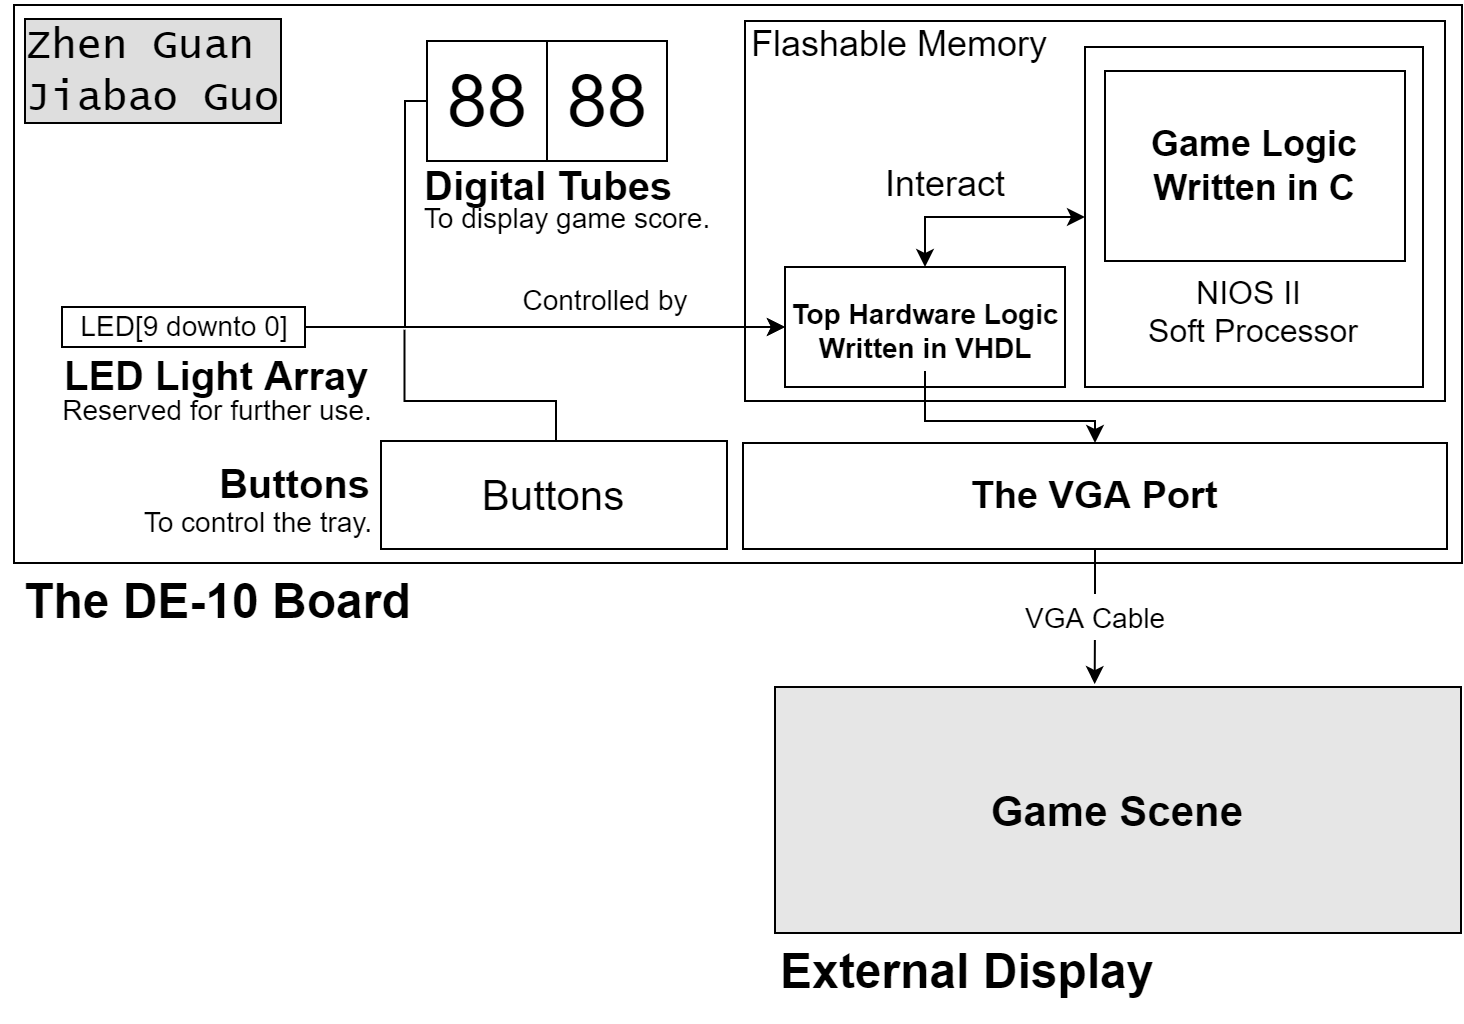
\includegraphics[width=0.7\textwidth]{imageset/diag_1.drawio} %[width=2.5in]
    \caption{Architecture of project.}
    \label{fig0}
\end{figure*}

\begin{figure*}[htbp] %h
    \centering
    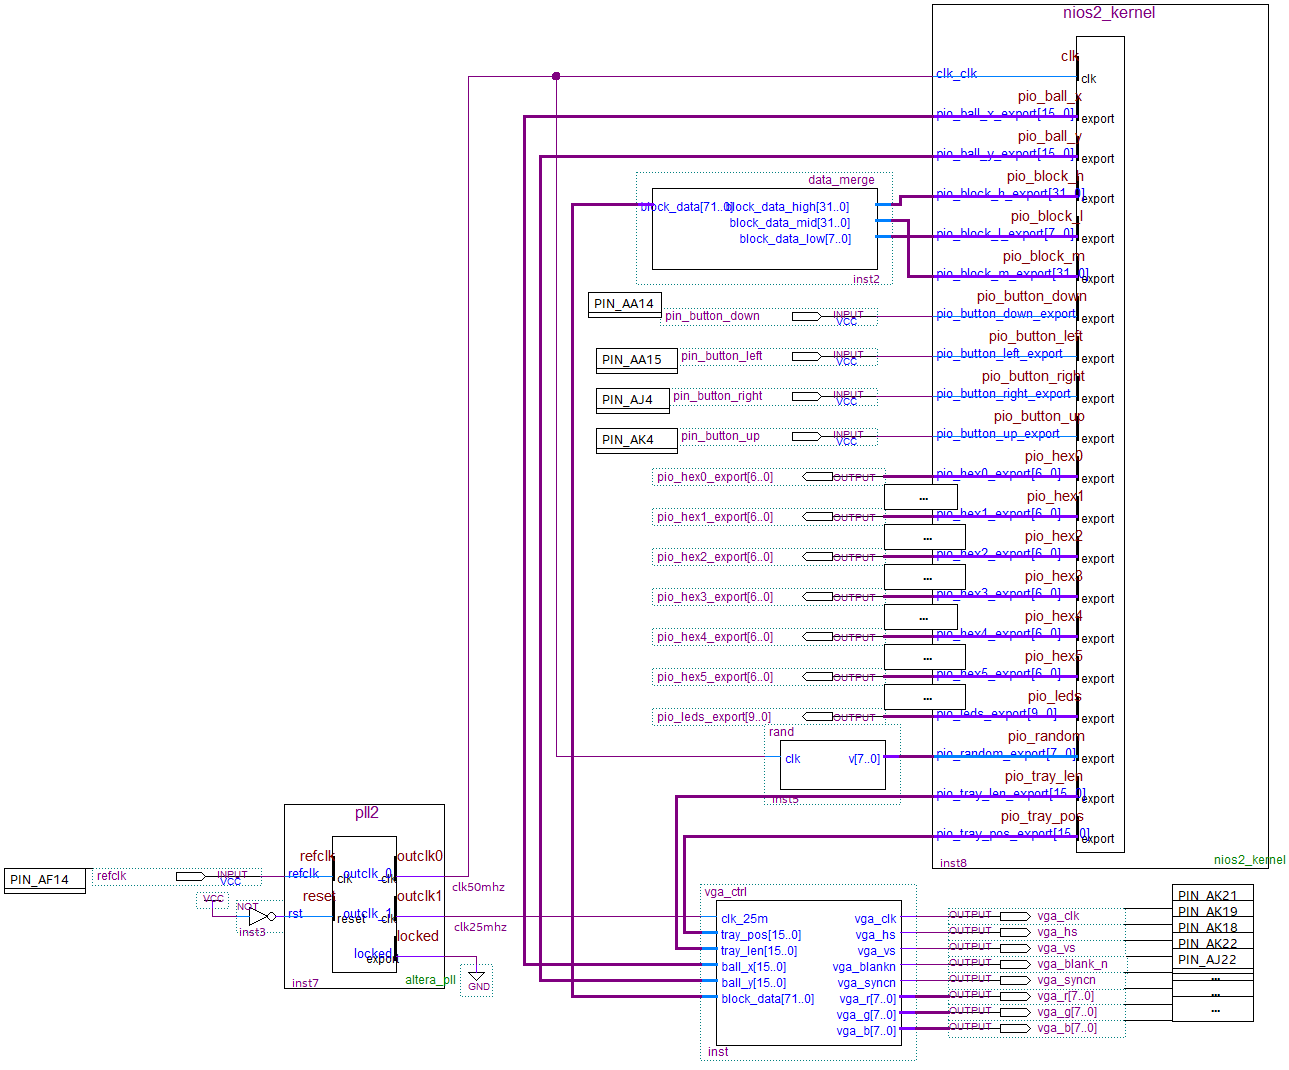
\includegraphics[width=0.8\textwidth]{imageset/top_level} %[width=2.5in]
    \caption{Top-level design of project.}
    \label{fig_top_level}
\end{figure*}

\begin{figure*}[htbp] %h
    \centering
    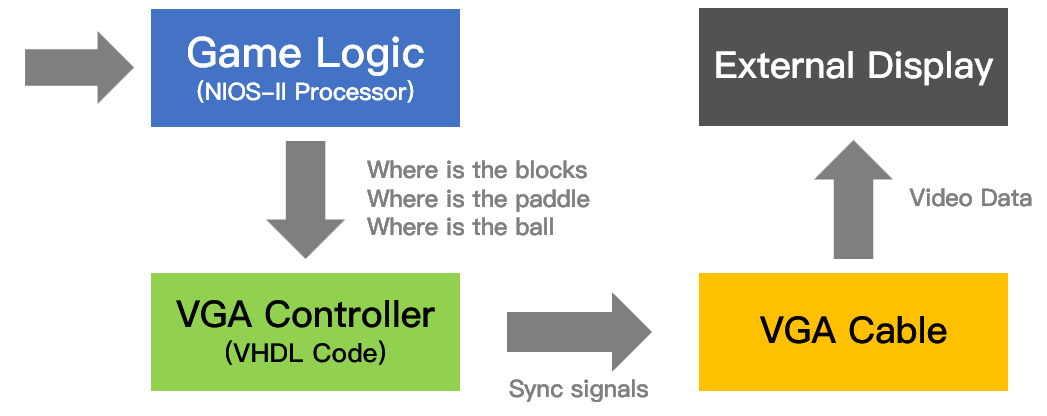
\includegraphics[width=0.7\textwidth]{imageset/arch_clear} %[width=2.5in]
    \caption{Architecture of project (Clearer Version).}
    \label{fig1}
\end{figure*}

Fig. \ref{fig0} is a coarse outline of our project. Since the entire game is based on NIOS, the C programming language will be the major way to illustrate the game logic instead of VHDL.

In the fig. \ref{fig0}, 
\begin{itemize}
    \item The ditigal tubes is used to display the game score,
    \item The buttons to control the paddle, the NIOS-II processor to run the game logic,
    \item Then, VHDL codes is used to convert the game scene into VGA signals,
    \item The LED Light Arrays are not used as planned.
\end{itemize}

The game logic was written in C, and where we used VHDL was only on controlling the VGA port, because only hardware description language (the HDL) have the direct access to the high frequency clock and achieve the synchronized programming.

Fig. \ref{fig_top_level} shows the top level of the project. It is a BDF (Block Diagram File) in Quartus II, and it is a very good way to visualize the design of the project. The BDF is essentially a clearer way to represent a VHDL/Verilog HDL/Other HDLs that is specifically used for top level logics that wiring every components together. From this figure, we can extract following information:
\begin{itemize}
    \item \textbf{The input/outputs of the NIOS-II processor.} This includes all data structures that used in the game logic, and will be explained later;
    \item \textbf{The input/outputs of the VGA port.} This includes all signals that used in the VGA port, and will be explained later;
    \item \textbf{The input/outputs of the Phase-locked loop.} This includes all signals that used in the PLL, an external IP core. The PLL will also be explained later.
\end{itemize}

\subsection{Data Structures}
\subsubsection{Clocks}
There are 2 clocks in the design:
\begin{itemize}
    \item \textbf{The 50MHz clock.} This clock is used to drive the game logic, and it is connected to the NIOS-II processor.
    \item \textbf{The 25MHz clock.} This clock is used to drive the VGA display to work as 640x480@60Hz, and it is connected to the VGA port.
\end{itemize}

\subsubsection{X and Y Axis of Ball}
Both $ball\_x$ and $ball\_y$ are 16-bit unsigned integer.

There is a special 2D coordinate system defined as following:

\begin{itemize}
    \item \textbf{The origin (Zero Point).} The origin point (0,0) is the \textbf{LEFT TOP CORNER} of the screen.
    \item \textbf{X axis.} Also known as the \textbf{Horizontal axis}, goes from LEFT to RIGHT, range from 0 to 640.
    \item \textbf{X axis.} Also known as the \textbf{Vertical axis}, goes from TOP to BOTTOM, range from 0 to 480.
\end{itemize}

This coordinate system is same as the windows in Microsoft Windows Operating System.


\subsubsection{Blocks Data}
The blocks data is an array of 8-bit unsigned integer with length 9, that is, $blocks\_data$[71 downto 0] or $alt\_u8$ $blocks\_data$[9].

For example,

\begin{center}
\begin{tabular}{c|c|c|c|c|c|c|c|c}
      & \textbf{0} & \textbf{1} & \textbf{2} & 
      \textbf{3} & \textbf{4} & \textbf{5} &
      \textbf{6} & \textbf{7} \\ 
    \hline
    \textbf{0} & 0 & 0 & 0 & 0 & 0 & 0 & 0 & 0 \\
    \hline
    \textbf{1} & 0 & 1 & 0 & 1 & 0 & 1 & 0 & 0 \\
    \hline
    \textbf{2} & 0 & 0 & 1 & 0 & 1 & 0 & 0 & 0 \\
    \hline
    \textbf{3} & 0 & 0 & 0 & 1 & 0 & 0 & 0 & 0 \\
    \hline
    \textbf{4} & 0 & 0 & 0 & 0 & 0 & 0 & 0 & 0 \\
    \hline
    \textbf{5} & 0 & 0 & 0 & 0 & 0 & 0 & 0 & 0 \\
    \hline
    \textbf{6} & 0 & 0 & 0 & 0 & 0 & 0 & 0 & 0 \\
    \hline
    \textbf{7} & 0 & 0 & 0 & 0 & 0 & 0 & 0 & 0 \\
    \hline
    \textbf{8} & 0 & 0 & 0 & 0 & 0 & 0 & 0 & 0
\end{tabular}        
\end{center}

represents that there are 3 blocks in the second row, 2 blocks in the third row and 1 block in the forth row, no blocks in other places.

For another example, regarding the blocks distribution in the fig. \ref{fig_gameplay}, the corresponding blocks data will be: 

\begin{center}
\begin{tabular}{c|c|c|c|c|c|c|c|c}
        & \textbf{0} & \textbf{1} & \textbf{2} & 
        \textbf{3} & \textbf{4} & \textbf{5} &
        \textbf{6} & \textbf{7} \\ 
    \hline
    \textbf{0} & 0 & 1 & 0 & 0 & 0 & 0 & 0 & 0 \\
    \hline
    \textbf{1} & 0 & 0 & 1 & 0 & 0 & 0 & 0 & 0 \\
    \hline
    \textbf{2} & 0 & 0 & 0 & 1 & 0 & 0 & 0 & 0 \\
    \hline
    \textbf{3} & 1 & 0 & 1 & 0 & 0 & 0 & 0 & 0 \\
    \hline
    \textbf{4} & 0 & 1 & 0 & 0 & 0 & 0 & 0 & 0 \\
    \hline
    \textbf{5} & 1 & 0 & 1 & 0 & 1 & 0 & 1 & 0 \\
    \hline
    \textbf{6} & 0 & 0 & 0 & 0 & 0 & 0 & 0 & 0 \\
    \hline
    \textbf{7} & 0 & 0 & 0 & 0 & 0 & 0 & 1 & 0 \\
    \hline
    \textbf{8} & 0 & 1 & 0 & 1 & 0 & 1 & 0 & 0
\end{tabular}        
\end{center}

Representing in flat, then we have 

$blocks\_data$[71 downto 0]$=$ 

\begin{center}
    ``010000000010000000010000101000000100
     000010101010000000000000001001010100''
\end{center}

\subsubsection{Button Signals}
$button\_left$, $button\_up$, $button\_down$, $button\_right$ are four 1-bit $std\_logic$s (button signals), corresponding to fig. \ref{fig_gameplay},  from left to right  respectively, \textbf{having a inversed logic that 0 represents ``Pressed'' and 1 represents ``Not Pressed''.} Their names are from the previous design (Guess My Number) and they are not standing for 4 directions now.

The inverted logic is because keeping a signal high is easier than keeping low. This avoids a lot of accidentally-triggers.

\subsubsection{Hex-es}
$hex$[0]~$hex$[5] are 6 digital tubes. Each of them is a 7-bit unsigned integer, or a 7-bit $std\_logic\_vector$. 

\begin{figure}[h] %h
    \centering
    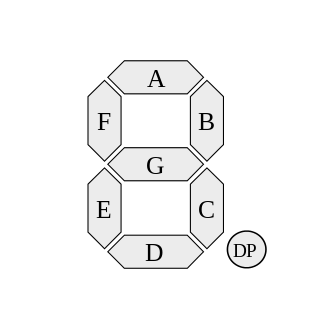
\includegraphics[width=0.45\textwidth]{imageset/seg7}
    \caption{
        7-Segment Digital Tube. \cite{bib_7seg}.
    }
    \label{fig_7seg}
\end{figure}

A digital tube is represented in "GFEDCBA" format, with every bit inverted that 1 means OFF and 0 means ON. For example, "0000000" represents "8", "0110000" represents "3", "0001000" represents "A".

\subsubsection{Tray Position and Length}
Both $tray\_len$ and $tray\_pos$ are 16-bit unsigned integers. The tray, or call it paddle, is vertically fixed on the $y=$SCREEN\_HEIGHT $-$ 52, and its X coordinate of left side is represented by $tray\_pos$.

The $tray\_len$ stores the length of the paddle, in pixels. The longer the paddle is, the easier to catch the ball, the easier the game is.

\subsection{Hardware Side: Pseudo-random Number Generator}
With a high frequency clock it is easy to generate random numbers. The random number generator in our system is actually an 8-bit counter. Along with the clock, the counter counts from 0 to 127 and then restart from 0. The user hit the ``Start Game'' button at unpredictable time, therefore the value in the counter is also unpredictable, but in a known range.

This module is not used in this project due to the change of the project subject, but is reserved for further use because it is simple and effective. It was useful in previous subject ``Guess My Number Game based on NIOS-II Soft Processor''.

\subsection{Hardware Side: Data Merger}
There is a limitation on the NIOS-II processor that we can not transmit more than 32-bit data in a single PIO port. However, although we compressed our blocks data to the extreme, it still occupies 72 bits. To transmit the blocks data we had to split it into a 32+32+8 form, that are high 32-bit, middle 32-bit and low 8-bit. After that, we did bitwise concatenation to restore the blocks data. 

For example, if we have

$blocks\_data$[71 downto 0]$=$ 

\begin{center}
    ``010000000010000000010000101000000100
     000010101010000000000000001001010100''
\end{center}

then 

$blocks\_data\_high32$[71 downto 40]$=$ 

\begin{center}
    ``01000000001000000001000010100000''
\end{center}

$blocks\_data\_mid32$[39 downto 8]$=$ 

\begin{center}
    ``01000000101010100000000000000010''
\end{center}

$blocks\_data\_low8$[7 downto 0]$=$ 

\begin{center}
    ``01010100''
\end{center}

Finally, to restore the original data, we do bitwise concatenation:

\lstset{
    columns=fixed,
    numbers=left,
    numberstyle=\tiny\color{gray},
    frame=lrtb,
    backgroundcolor=\color[RGB]{245,245,244},
    numberstyle=\footnotesize\color{darkgray},           
    commentstyle=\it\color[RGB]{0,96,96},
    stringstyle=\rmfamily\slshape\color[RGB]{128,0,0},
    showstringspaces=false,
    language=vhdl,
}
\begin{lstlisting}
    blocks_data <= 
        blocks_data_h 
        & blocks_data_m 
        & blocks_data_l;
\end{lstlisting}

There are also bitwise reverse problem: we found that the data in the PIO output is not in the same order as input. So we had to reverse the data before passing in the PIO port:

\lstset{
    columns=fixed,
    numbers=left,
    numberstyle=\tiny\color{gray},
    frame=lrtb,
    backgroundcolor=\color[RGB]{245,245,244},
    numberstyle=\footnotesize\color{darkgray},           
    commentstyle=\it\color[RGB]{0,96,96},
    stringstyle=\rmfamily\slshape\color[RGB]{128,0,0},
    showstringspaces=false,
    language=c,
}
\begin{lstlisting}
alt_u32* gp_block_data_high = reverse_bit(
    (alt_u32*)(data + 0) );
alt_u32* gp_block_data_mid = reverse_bit(
    (alt_u32*)(data + 4) );
alt_u8* gp_block_data_low = reverse_bit(
    (alt_u8*)(data + 8) );
\end{lstlisting}

Having the defination of $reverse\_bit$ that 

\begin{lstlisting}
alt_u32 reverse_bit(alt_u32 a) {
    a = ((a >> 1) & 0x55555555) 
        | ((a & 0x55555555) << 1);
    a = ((a >> 2) & 0x33333333) 
        | ((a & 0x33333333) << 2);
    a = ((a >> 4) & 0x0F0F0F0F) 
        | ((a & 0x0F0F0F0F) << 4);
    a = ((a >> 8) & 0x00FF00FF) 
        | ((a & 0x00FF00FF) << 8);
    a = ( a >> 16) | (a << 16);
    return a; }
\end{lstlisting}

\textbf{The reverse\_bit function is generated by Github Copilot.}

\subsection{Hardware Side: VGA Controller}
It requires a group of specific values to make the monitor run on a certain resolution but we could not find one from the user manual. Finally we consulted the internet (https://electronics.stackexchange.com/questions/532192/intel-de1-soc-vga-controller-in-vhdl) for the correct code to generate Hsync and Vsync signals.


\subsection{Software Side: Chrono, CoreGame, CoreIO and Logging}
\begin{figure}[h] %h
    \centering
    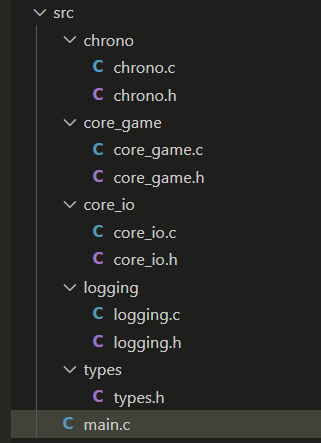
\includegraphics[height=2in]{imageset/tree}
    \caption{Source Tree of Sofrware Side}
    \label{fig_source_tree}
\end{figure}

The design of software side (game logic side) is divided into 5 parts.

\subsubsection{Chrono}
The chrono module seals \emph{alt\_types.h} and provide a \emph{msleep} function to sleep in milliseconds.

In addition, this module provide a convenient macro that 
\lstset{
    columns=fixed,
    numbers=right,
    numberstyle=\tiny\color{gray},
    frame=lrtb,
    backgroundcolor=\color[RGB]{245,245,244},
    numberstyle=\footnotesize\color{darkgray},           
    commentstyle=\it\color[RGB]{0,96,96},
    stringstyle=\rmfamily\slshape\color[RGB]{128,0,0},
    showstringspaces=false,
    language=c,
}
\begin{lstlisting}
#define time_warp(
    variable, 
    kiloperiod, 
    proc) \
if ((++(variable)) >= 1000*(kiloperiod))\
    { variable=0; proc; }
\end{lstlisting}

This is an implement of frequency divider. The use of \emph{time\_warp} is easy:

\begin{lstlisting}
// Requires a static variable.
static int i = 0;

// Some kind of loops
for (;;) {
    time_warp(i, 25, {
        if (is_button_left_pressed()) {
            // No fluctuations here!
            // Do something.
        }
    });    
}
\end{lstlisting}

This is a 25000 divider that slows down the clock by approximately 25000 times (Of course there are no real ``clk''s, but this do helps with the fluctuation of the button).

\subsubsection{CoreGame}
This module handles the real main game logic, including ball movement, ball collision detection, state transitions, level(stage) designs, flashed text logics, etc. For detailed information please refer to the source code (core\_game.c).

\subsubsection{CoreIO}
This module handles all interactions with the PIO port, for example, digital tubes write-back, ball positions write-back, charater-to-segment-data converter, etc. This module is also designed to be the only one that interacting with the PIO. For detailed information please refer to the source code (core\_io.c).

\subsubsection{Logging}
This module is only for logging, providing $log\_info$ and $log\_error$. In executables running on NIOS-II, the standard output stream $stdout$ is read by the UART debug port and displayed through nios2-terminal. For detailed information please refer to the source code (logging.c).

\subsubsection{Types}
This is a header file providing TRUE, FALSE and UNREFERENCED\_PARAMETER support.
\lstset{
    columns=fixed,
    numbers=left,
    numberstyle=\tiny\color{gray},
    frame=lrtb,
    backgroundcolor=\color[RGB]{245,245,244},
    numberstyle=\footnotesize\color{darkgray},           
    commentstyle=\it\color[RGB]{0,96,96},
    stringstyle=\rmfamily\slshape\color[RGB]{128,0,0},
    showstringspaces=false,
    language=c,
}
\begin{lstlisting}
    typedef alt_u8  BOOL;
    #define TRUE    (1)
    #define FALSE   (0)
    #define UNREFERENCED(x) ((void)(x))
\end{lstlisting}


\subsection{State Transitions}

\textbf{Design Thoughts:} In order to reduce the design complexity and make state transition more explicit, we intend to design out ASM chart in ``One-Hot Encoding'' form and it would be implemented as a prototype of ``Moore State Machine''.

\textbf{List of Notations:} We assume that 
\begin{align*}
    \text{State } &IDLE &= S_0 \\ 
    \text{State } &IN\_GAME &= S_1 \\
    \text{State } &WIN &= S_2 \\
    \text{State } &LOSE &= S_3 \\
    \text{State } &OVER &= S_4
\end{align*}

and also abbreviations:
\begin{align*}
    reset &= r \\ 
    cheat &= c \\
    \text{``Press Any Key''} &= PAK \\ 
    \text{``Good Job''} &= GJ \\
    \text{``Game Clear''} &= GC \\
    \text{``Better Next Time''} &= BNT
\end{align*}

where $cheat$ represents the Cheat Button mentioned in the Section I.

\pagebreak

\textbf{State Assginments:}

\begin{center}
\begin{tabular}{|c|ccccc|}
    \hline
    State & $Q_1$ & $Q_2$ & $Q_3$ & $Q_4$ & $Q_5$ \\ 
    \hline
    $S_0$ & 0 & 0 & 0 & 0 & 1 \\
    $S_1$ & 0 & 0 & 0 & 1 & 0 \\
    $S_2$ & 0 & 0 & 1 & 0 & 0 \\
    $S_3$ & 0 & 1 & 0 & 0 & 0 \\
    $S_4$ & 1 & 0 & 0 & 0 & 0 \\
    \hline
\end{tabular}        
\end{center}


\subsubsection{ASM Chart}
\begin{figure}[h] %h
    \centering
    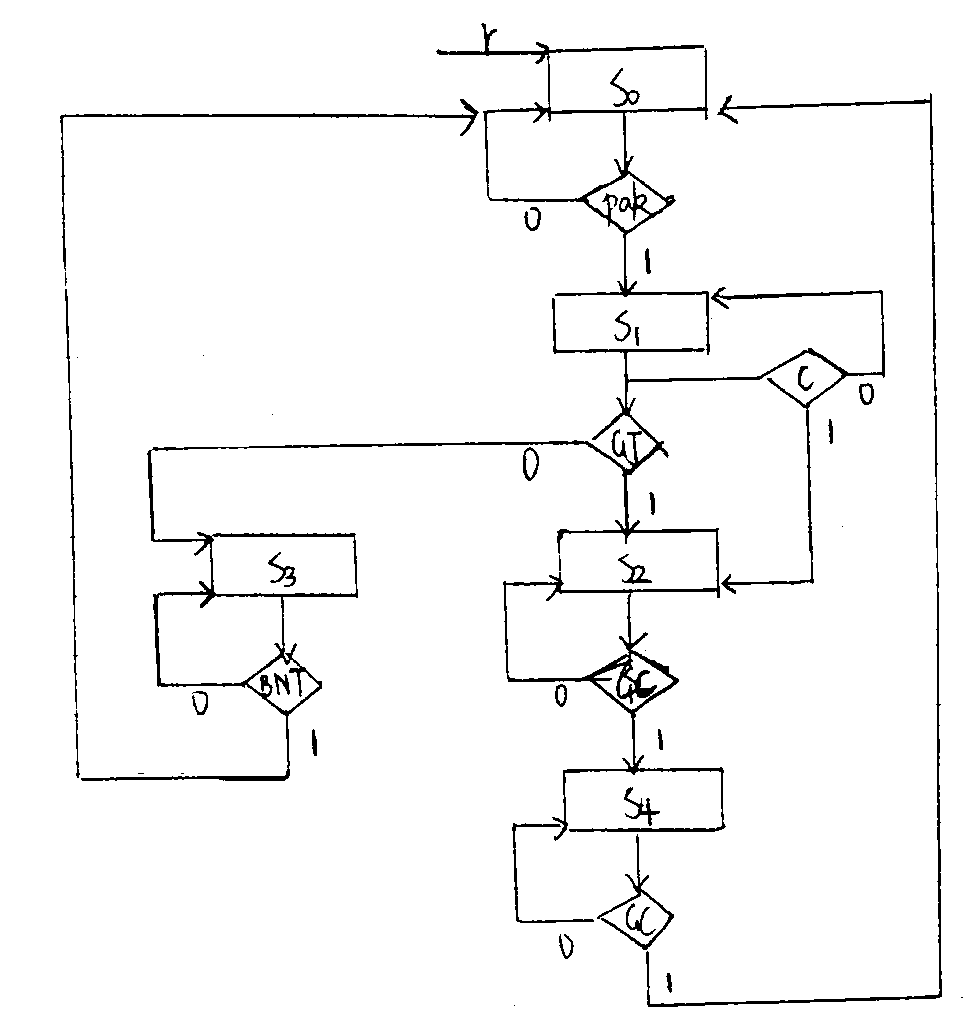
\includegraphics[width=0.45\textwidth]{imageset/asm}
    \caption{The ASM chart of the design.}
    \label{fig_asm}
\end{figure}

\textbf{Fig. \ref{fig_asm} is the ASM chart of the design.} This figure may be laid on other pages because of some typesetting policies of \LaTeX.


\subsubsection{State Transition Diagram}
\begin{figure}[h] %h
    \centering
    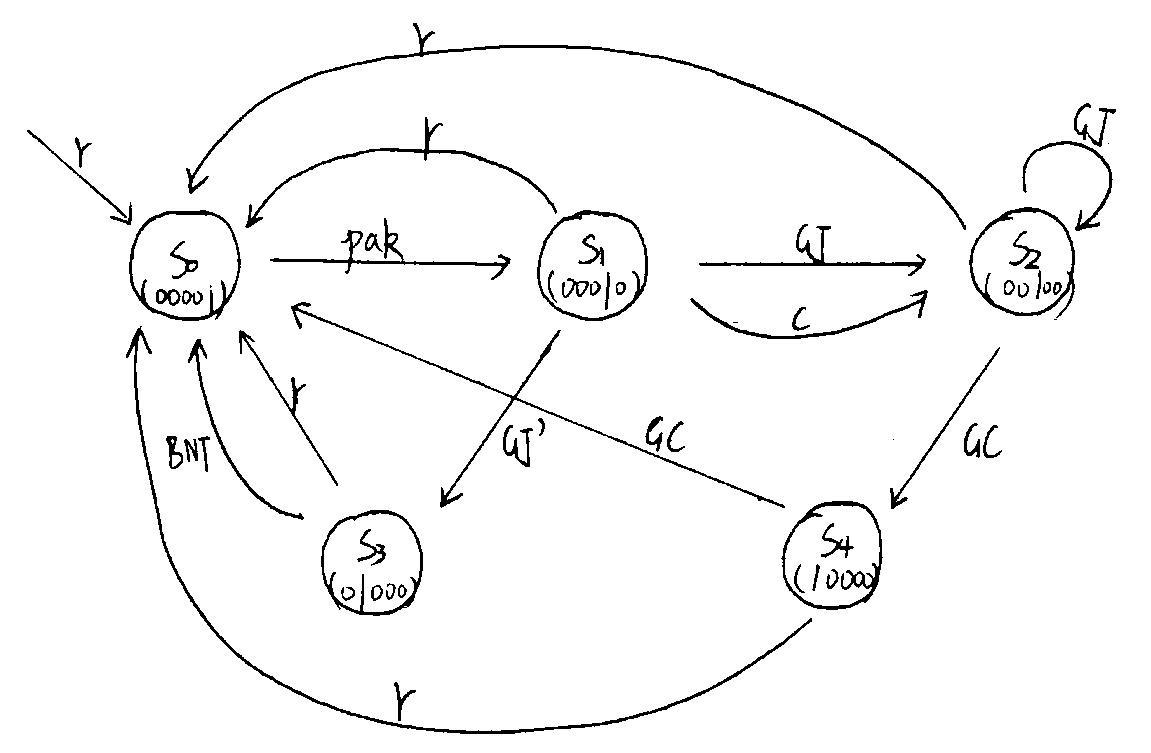
\includegraphics[width=0.45\textwidth]{imageset/state}
    \caption{The state transition diagram of the design.}
    \label{fig_state}
\end{figure}

\textbf{Fig. \ref{fig_state} is the state transition diagram of the design.} This figure may be laid on other pages because of some typesetting policies.

%%%%%%%%%%%%%%%%%%%%%%%%%%%%%%%%%%%%%%%%%%%%%%
%%%%%%%%%%%%%%%%%%%%%%%%%%%%%%%%%%%%%%%%%%%%%%
%%%%%%%%%%%%%%%%%%%%%%%%%%%%%%%%%%%%%%%%%%%%%%
%%%%%%%%%%%%%%%%%%%%%%%%%%%%%%%%%%%%%%%%%%%%%%
%%%%%%%%%%%%%%%%%%%%%%%%%%%%%%%%%%%%%%%%%%%%%%
%%%%%%%%%%%%%%%%%%%%%%%%%%%%%%%%%%%%%%%%%%%%%%
%%%%%%%%%%%%%%%%%%%%%%%%%%%%%%%%%%%%%%%%%%%%%%
%%%%%%%%%%%%%%%%%%%%%%%%%%%%%%%%%%%%%%%%%%%%%%
%%%%%%%%%%%%%%%%%%%%%%%%%%%%%%%%%%%%%%%%%%%%%%
%%%%%%%%%%%%%%%%%%%%%%%%%%%%%%%%%%%%%%%%%%%%%%
%%%%%%%%%%%%%%%%%%%%%%%%%%%%%%%%%%%%%%%%%%%%%%
%%%%%%%%%%%%%%%%%%%%%%%%%%%%%%%%%%%%%%%%%%%%%%

\section{Profiling of Design}

\subsection{QuestaSim Simulation}
QuestaSim is a newer version of ModelSim with 64-bit machine support.  we are using QuestaSim for the testbench on hardware side.

The test project is located at the /sim path of project root.

As you can see in fig. \ref{fig_sim0}, the simulation is targeted to 3 components: 
\begin{itemize}
    \item VGA Controller,
    \item Data Merger,
    \item Random Number Generator.
\end{itemize}

\begin{figure}[h] %h
    \centering
    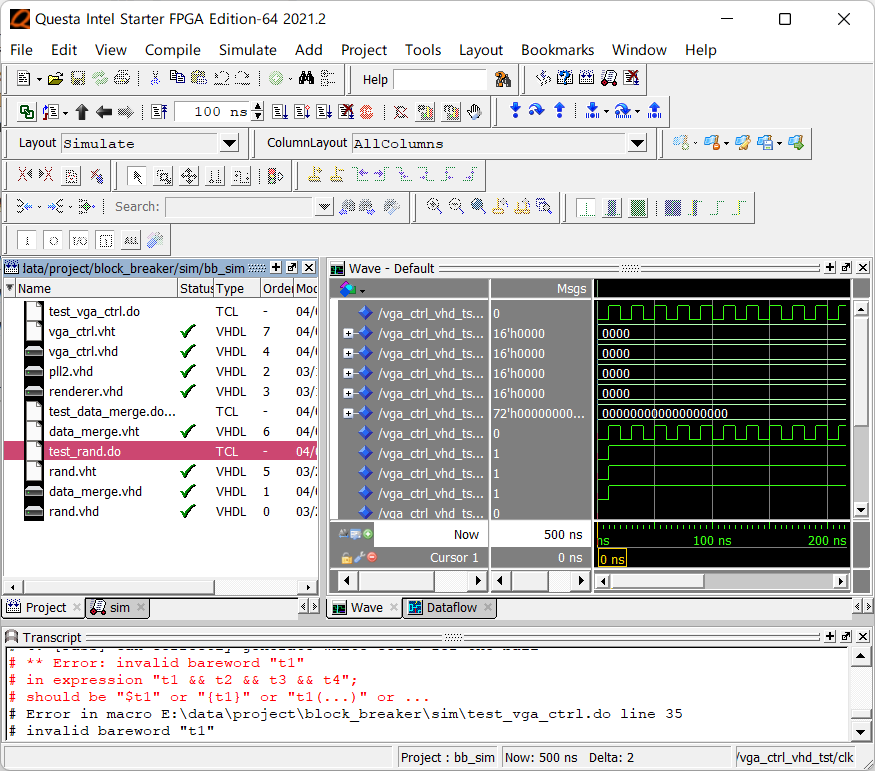
\includegraphics[width=0.45\textwidth]{imageset/sim0}
    \caption{QuestaSim. Can be launched via command ``vsim''}
    \label{fig_sim0}
\end{figure}


\subsection{Automatic Test Report Generation based on TCL Script and QuestaSim}
We designed 3 TCL scripts for the 3 test subjects (VGA Controller, Data Merger and Random Number Generator).

As of fig. \ref{fig_sim1}, after executing each of the scripts, the test report is generated automatically, a message box will be popped up, showing an overall PASS/FAIL signal for each component, followed with a list of testcases and the PASS/FAIL status for each of them, without having to check the waveform manually) by simply clicking the menu item ``Execute'' in the GUI.

For detailed TCL script code please refer to the source code (/sim/test\_rand.do, /sim/test\_vga\_ctrl.do and /sim/test\_data\_merge.do).

\begin{figure}[h] %h
    \centering
    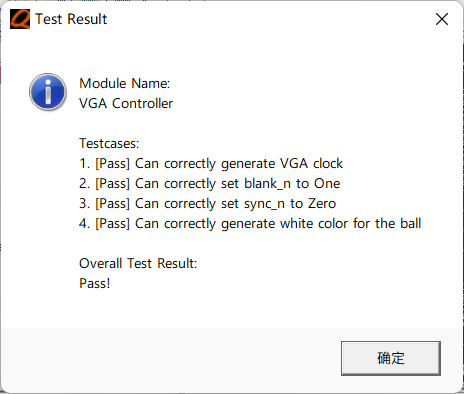
\includegraphics[width=0.45\textwidth]{imageset/testresult}
    \caption{Test result generated by TCL Script. The message box is shown by calling WinAPI ``MessageBoxA/W'' which is localized according to the host machine's language. The Chinese text in the button represents the meanning of ``Confirm'' or ``OK''.}
    \label{fig_sim1}
\end{figure}


\subsection{Discuss on Software Testing Framework}
Existing C/C++ testing frameworks are not suitable for our testing needs. The list of frameworks we had evaluated are:
\begin{itemize}
    \item \textbf{CTest}. Not suitable bacause this is an executable-level test based on CMake. The target platform (NIOS-II CPU Architecture) does not support this.
    \item \textbf{CUnit}. Not suitable bacause implementing a CUnit requires adding external libraries and this is not a good selection for embedded development. Although we can use macros to generate a kind of ``Release Build'' that compiles without testing framworks, this is still causing too much code change.
    \item \textbf{QuestaSim on NIOS-II}. This is an official method to run QuestaSim on projects using NIOS-II. However, this requires a long list of steps to initiate and currently there are neither enough documentation on this, nor enough related discussions on any forums. We can not use this high risk method.
\end{itemize}

We need a more flexible testing framework that:
\begin{itemize}
    \item Has nearly no change to existing code, to ensure maximum compatibility;
    \item Using no third-party libraries, so that it can work well with embedded development;
    \item Or can be runned directly on the development environment, without having to run on the FPGA board, such as QuestaSim.
\end{itemize}

\textbf{Taking the above into consideration, we have written a very simple C testing framework for this project only, temperarily called ``Easy Test'',} with the following advantages:

\begin{itemize}
    \item Has no code change to the existing project;
    \item Using only pure C and standard IO (stdio.h);
    \item Based on CMake that allows module-level testing and easy to manage the compiler parameters;
    \item Running the test directly on the developemnt environment, without having to turn on the FPGA board.
\end{itemize}

Regarding the source code of Easy Test please also refer to the files that submitted along with this report (/test/framework/easytest.c).

\subsection{Introduction to ``Fake Environment''}
\begin{figure}[h] %h
    \centering
    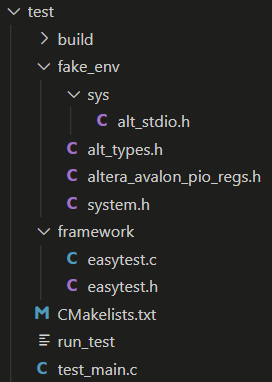
\includegraphics[height=2in]{imageset/test}
    \caption{Easy Test and ``Fake Environment''}
    \label{fig_sim2}
\end{figure}


We also created \textbf{a fake NIOS-II runtime library} to work with the testing, temperarily called ``Fake Environment''. This is creating a partial NIOS-II runtime on the PC but blocking all hardware-related operations. 

For example, \emph{altera\_avalon\_pio\_regs.h}, which is an important NIOS-II runtime library, providing IO operations for the PIOs, while in the fake environment, all IO operations will do nothing but still return a legal value. This has no actual impact to the testing, because according to our design of the software side, unable to access the hardware will not influence the state transition.


\subsection{Test Result}
\begin{figure}[h] %h
    \centering
    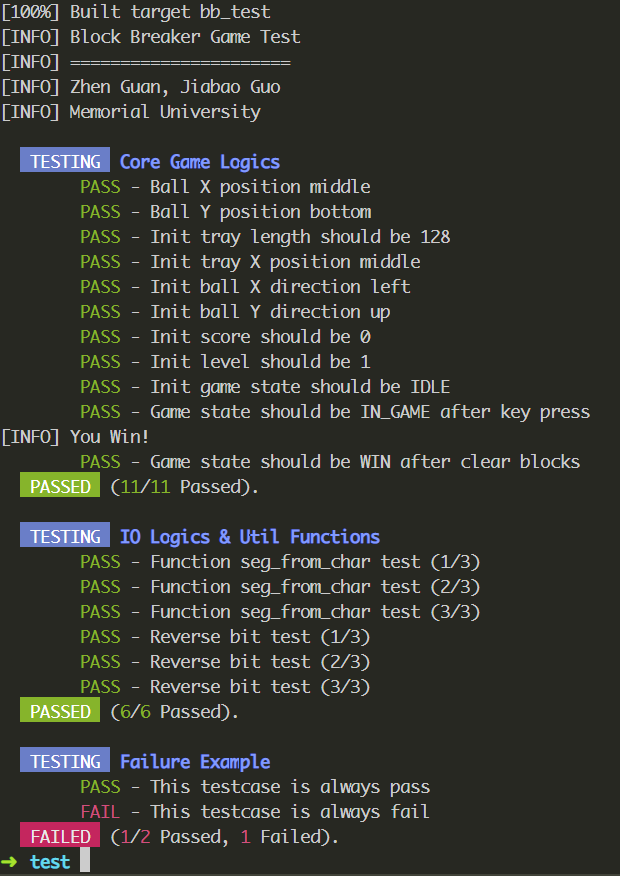
\includegraphics[width=0.45\textwidth]{imageset/test2}
    \caption{
        Software Testing using Easy Test. \textbf{The last test is failed because its a test to show what a failed test looks like.}
    }
    \label{fig_sim3}
\end{figure}

\begin{figure}[h] %h
    \centering
    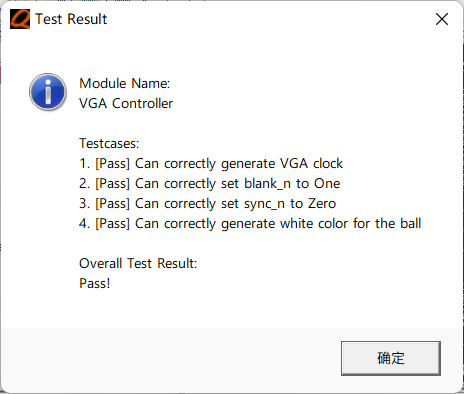
\includegraphics[width=0.45\textwidth]{imageset/testresult}
    \caption{Test Report of VGA Controller}
    \label{fig_sim4}
\end{figure}

\begin{figure}[h] %h
    \centering
    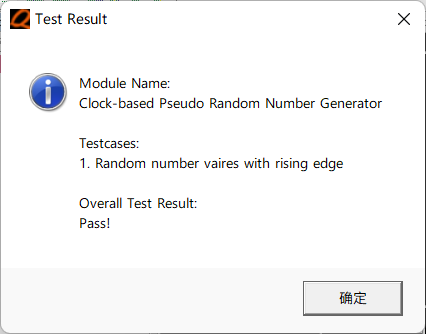
\includegraphics[width=0.45\textwidth]{imageset/test3}
    \caption{Test Report of Rand Generator}
    \label{fig_sim5}
\end{figure}

\begin{figure}[t] %h
    \centering
    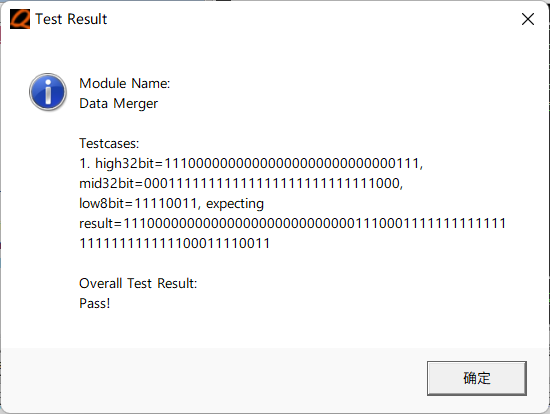
\includegraphics[width=0.45\textwidth]{imageset/test4}
    \caption{Test Report of Data Merger}
    \label{fig_sim6}
\end{figure}



Fig. \ref{fig_sim3} shows the test result of the software side. The test result is generated by \textbf{Easy Test}.

Fig. \ref{fig_sim4} shows the test result of the VGA Controller.

Fig. \ref{fig_sim5} shows the test result of the Rand Generator.

Fig. \ref{fig_sim6} shows the test result of the Data Merger.

All the tests were finished in very short time, and passed all testcases. This is identical to the actual run on the FPGA board. The gameplay is seamless and had a very good user experience and very challenging difficulty.

We are trying to continue to improve the testing framework, making it compatible with any future works. We are also trying to improve the user experience, by providing a more friendly interface and a more intuitive testing process. 

\pagebreak

\section{Appendix}


%%%%%%%%%%%%%%%%%%%%%%%%%%%%%%%%%%%%%%%%%%%%%%
%%%%%%%%%%%%%%%%%%%%%%%%%%%%%%%%%%%%%%%%%%%%%%
%%%%%%%%%%%%%%%%%%%%%%%%%%%%%%%%%%%%%%%%%%%%%%
%%%%%%%%%%%%%%%%%%%%%%%%%%%%%%%%%%%%%%%%%%%%%%
%%%%%%%%%%%%%%%%%%%%%%%%%%%%%%%%%%%%%%%%%%%%%%
%%%%%%%%%%%%%%%%%%%%%%%%%%%%%%%%%%%%%%%%%%%%%%
%%%%%%%%%%%%%%%%%%%%%%%%%%%%%%%%%%%%%%%%%%%%%%
%%%%%%%%%%%%%%%%%%%%%%%%%%%%%%%%%%%%%%%%%%%%%%
%%%%%%%%%%%%%%%%%%%%%%%%%%%%%%%%%%%%%%%%%%%%%%
%%%%%%%%%%%%%%%%%%%%%%%%%%%%%%%%%%%%%%%%%%%%%%
%%%%%%%%%%%%%%%%%%%%%%%%%%%%%%%%%%%%%%%%%%%%%%
%%%%%%%%%%%%%%%%%%%%%%%%%%%%%%%%%%%%%%%%%%%%%%

\begin{thebibliography}{20}
    \bibitem{bib_nios2}
    Altera. \emph{Nios II Embedded Processor Backgrounder} (PDF), https://www.intel.com/content/dam/www/programmable/us/en/pdfs/liter\\ature/pr/nios2\_backgrounder.pdf.

    \bibitem{bib_7seg}
    Tan, Yin, H., Xu, J., Jiang, F., Chen, T., \& Li, W. (2021). \emph{Design and Manufacture of Programmable Electrochromic Digital Tube}. In Advances in Graphic Communication, Printing and Packaging Technology and Materials (pp. 366-372). Springer Singapore. https://doi.org/10.1007/978-981-16-0503-1\_54

    \bibitem{bib_fpgamethod}
    E. Monmasson and M. N. Cirstea, \emph{FPGA Design Methodology for Industrial Control Systems—A Review}, in IEEE Transactions on Industrial Electronics, vol. 54, no. 4, pp. 1824-1842, Aug. 2007, doi: 10.1109/TIE.2007.898281.

    \bibitem{bib_neural}
    M. N. Cirstea, A. Dinu, J. Khor, and M. McCormick, \emph{Neural and Fuzzy Logic Control of Drives and Power Systems}. Oxford, U.K.: Elsevier, 2002.

    \bibitem{bib_vhdl}
    D. L. Perry, \emph{VHDL}. New York: McGraw-Hill, 2004.

    \bibitem{bib_fpgadrive}
    C. Cecati, \emph{Microprocessors for power electronics and electrical drives applications}, IEEE Ind. Electron. Soc. Newsl., vol. 46, no. 3, pp. 5-9, Sep. 1999.

    \bibitem{bib_fpgaarch}
    S. Brown, \emph{FPGA architectural research: A survey}, IEEE Des. Test. Comput., vol. 13, no. 4, pp. 9-15, Winter 1996.

    \bibitem{bib_fpgasites}
    Internet sites and on line journals dedicated to FPGAs, such as: “FPGA-FAQ”. [Online]. Available: http://www.fpga-faq.com/, “FPGA and Structured ASIC Journal,” http://www.fpgajournal.com/

    \bibitem{bib_vgafpga}
    Mishra, A. et al. (2018) \emph{VGA Application in Text Display Using FPGA}, in Intelligent Communication, Control and Devices. [Online]. Singapore: Springer Singapore. pp. 1575-1585.

    \bibitem{bib_statemachine}
    Gazi, O. \& Arli, A. C. (2021) \emph{State Machines using VHDL FPGA Implementation of Serial Communication and Display Protocols}. 1st ed. 2021. [Online]. Cham: Springer International Publishing.

    \bibitem{bib_vhdlstyle}
      Cohen, B. (1999) \emph{VHDL Coding Styles and Methodologies}. 2nd ed. 1999. [Online]. New York, NY: Springer US.
\end{thebibliography}

This report is at an end and thank you very much to review our work.

\end{document}

% hao nan a

% trigger a \newpage just before the given reference
% number - used to balance the columns on the last page
% adjust value as needed - may need to be readjusted if
% the document is modified later
%\IEEEtriggeratref{8}
% The "triggered" command can be changed if desired:
%\IEEEtriggercmd{\enlargethispage{-5in}}

% references section

% can use a bibliography generated by BibTeX as a .bbl file
% BibTeX documentation can be easily obtained at:
% http://mirror.ctan.org/biblio/bibtex/contrib/doc/
% The IEEEtran BibTeX style support page is at:
% http://www.michaelshell.org/tex/ieeetran/bibtex/
%\bibliographystyle{IEEEtran}
% argument is your BibTeX string definitions and bibliography database(s)
%\bibliography{IEEEabrv,../bib/paper}
%
% <OR> manually copy in the resultant .bbl file
% set second argument of \begin to the number of references
% (used to reserve space for the reference number labels box)






% An example of a floating figure using the graphicx package.
% Note that \label must occur AFTER (or within) \caption.
% For figures, \caption should occur after the \includegraphics.
% Note that IEEEtran v1.7 and later has special internal code that
% is designed to preserve the operation of \label within \caption
% even when the captionsoff option is in effect. However, because
% of issues like this, it may be the safest practice to put all your
% \label just after \caption rather than within \caption{}.
%
% Reminder: the "draftcls" or "draftclsnofoot", not "draft", class
% option should be used if it is desired that the figures are to be
% displayed while in draft mode.
%
%\begin{figure}[!t]
%\centering
%\includegraphics[width=2.5in]{myfigure}
% where an .eps filename suffix will be assumed under latex, 
% and a .pdf suffix will be assumed for pdflatex; or what has been declared
% via \DeclareGraphicsExtensions.
%\caption{Simulation results for the network.}
%\label{fig_sim}
%\end{figure}

% Note that the IEEE typically puts floats only at the top, even when this
% results in a large percentage of a column being occupied by floats.


% An example of a double column floating figure using two subfigures.
% (The subfig.sty package must be loaded for this to work.)
% The subfigure \label commands are set within each subfloat command,
% and the \label for the overall figure must come after \caption.
% \hfil is used as a separator to get equal spacing.
% Watch out that the combined width of all the subfigures on a 
% line do not exceed the text width or a line break will occur.
%
%\begin{figure*}[!t]
%\centering
%\subfloat[Case I]{\includegraphics[width=2.5in]{box}%
%\label{fig_first_case}}
%\hfil
%\subfloat[Case II]{\includegraphics[width=2.5in]{box}%
%\label{fig_second_case}}
%\caption{Simulation results for the network.}
%\label{fig_sim}
%\end{figure*}
%
% Note that often IEEE papers with subfigures do not employ subfigure
% captions (using the optional argument to \subfloat[]), but instead will
% reference/describe all of them (a), (b), etc., within the main caption.
% Be aware that for subfig.sty to generate the (a), (b), etc., subfigure
% labels, the optional argument to \subfloat must be present. If a
% subcaption is not desired, just leave its contents blank,
% e.g., \subfloat[].


% An example of a floating table. Note that, for IEEE style tables, the
% \caption command should come BEFORE the table and, given that table
% captions serve much like titles, are usually capitalized except for words
% such as a, an, and, as, at, but, by, for, in, nor, of, on, or, the, to
% and up, which are usually not capitalized unless they are the first or
% last word of the caption. Table text will default to \footnotesize as
% the IEEE normally uses this smaller font for tables.
% The \label must come after \caption as always.
%
%\begin{table}[!t]
%% increase table row spacing, adjust to taste
%\renewcommand{\arraystretch}{1.3}
% if using array.sty, it might be a good idea to tweak the value of
% \extrarowheight as needed to properly center the text within the cells
%\caption{An Example of a Table}
%\label{table_example}
%\centering
%% Some packages, such as MDW tools, offer better commands for making tables
%% than the plain LaTeX2e tabular which is used here.
%\begin{tabular}{|c||c|}
%\hline
%One & Two\\
%\hline
%Three & Four\\
%\hline
%\end{tabular}
%\end{table}


% Note that the IEEE does not put floats in the very first column
% - or typically anywhere on the first page for that matter. Also,
% in-text middle ("here") positioning is typically not used, but it
% is allowed and encouraged for Computer Society conferences (but
% not Computer Society journals). Most IEEE journals/conferences use
% top floats exclusively. 
% Note that, LaTeX2e, unlike IEEE journals/conferences, places
% footnotes above bottom floats. This can be corrected via the
% \fnbelowfloat command of the stfloats package.


